\documentclass{scrartcl}
\usepackage[ansinew]{inputenc}
%\usepackage[T1]{fontenc}
%\usepackage[ngerman]{babel} % Neue Rechtschreibung
\usepackage{amsmath} % Verbesserter Mathesatz
\usepackage{amssymb}
\usepackage{graphicx}
\usepackage{listings}
\usepackage{color}

\parskip1ex

\lstset{language=Java}
\lstset{numbers=right, numberstyle=\tiny, numbersep=5pt, tabsize=3, breaklines=true}
\lstset{basicstyle=\small\ttfamily,stringstyle=\ttfamily, keywordstyle=\color{blue}\bfseries,commentstyle=\color{OliveGreen}}

\title{\begin{small}Manual\end{small}\\An ImageJ Plugin to Measure 3D Point Spread Functions (alpha)}
\date{November 2010}
\author{Janick Cardinale, \texttt{janick@inf.ethz.ch}\\MOSAIC Group, www.mosaic.inf.ethz.ch}
\begin{document}

\maketitle

\section{Introduction}
\label{sec:intro}
Subpixel-resolution image analysis often exploit knowledge about the imaging system to analyze the measurements (or \textit{observations}). Using prior knowledge enables more robust and accurate reconstructions of the hidden state than when just using observations. 

In light microscopy, the mapping from \textit{object space} to \textit{image space} is often modeled using a convolution of the true state with the point spread function (PSF) of the imaging system:
\[   
I = O * \textnormal{PSF} + \eta
\] 
where $\eta$ is a random variable accounting for noise, $I$ the image observed. $O$ is the \textit{model image} or \textit{object image}. It is an indicator function. Depending on the model used, $O$ indicates what object with what intensity is at a certain position in space.  The inverse problem of reconstructing the objects from the images using \textit{deconvolution} techniques is much easier when the PSF is known a-priori. 

When convolving a Dirac delta function $\delta$ with a kernel $K$, the result is $K$ itself since $\delta$ is the neutral element of the convolution operation. Thus, in fluorescence microscopy, imaging small fluorescent micro-spheres, also called \textit{beads}, as an approximation to a Dirac impulse, enables to observe the PSF of the system in the resulting image. For confocal microscopy, the PSF is of Gaussian-blob like shape.

This ImageJ plugin creates high resolution PSF images by averaging many bead images as well as exploiting the assumption that the point spread function is rotationally symmetric with respect to the axial axis (z-direction).

Note that in 3D microscopy the PSF may differ depending on the axial position of the emitting light source. This effect is neglected by the current implementation.

\section{Installation}
Copy the \texttt{mosaic\_plugins.jar} file to the ImageJs \texttt{plugins} directory. Restart ImageJ. The plugin can be launched from the \texttt{Mosaic} sub-menu in ImageJs plugin menu. 

The plugin handles 8-bit, 16-bit and 32-bit grayscale images or stacks. 

Prerequisites: At least Java 5.0 and ImageJ 1.36.

\section{How to use the plugin}
Open a 3D or 4D image stack in ImageJ. Please make sure to correctly set the number of slices per frame and the number of frames correctly in the image properties dialog (\texttt{Ctrl-P}). Also put the correct value for the pixel size and focal plane distance (preferably in nm). In the \texttt{Plugin$\rightarrow$Mosaic} menu, selecting the \texttt{PSF measure 3D} entry in the \texttt{Mosaic} sub-menue starts the plugin. 

A maximum intensity projection of your stack pops up. Then, select ImageJs point selection tool. Clicking on a bead while holding the \texttt{SHIFT} button creates a PSF map with the first measurement (the first measurement might take some time). Repeat this for all the good quality beads in your image. Do not select beads that are close to another bead. The PSF-map (see figure \ref{fig:psfmap}) created after each new measurement is averaging all the measurements taken so far. To remove a certain measurement, shift-click on the corresponding bead again.

\begin{figure}[h]
  \centering
  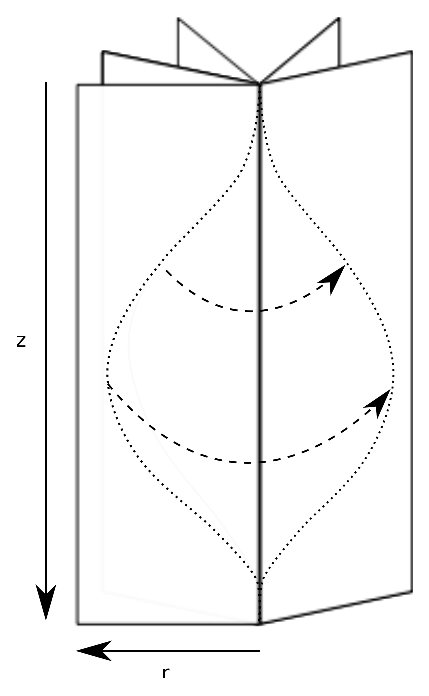
\includegraphics[width=0.8\textwidth]{psfmap} 
  \caption{ (a) Intensity isoline of the PSF: rotating the PSF map around the axial axis yields a 3D PSF. (b) A PSF map generated by measuring 20 beads. The beads were recorded by a spinning disk confocal microscope.
  \label{fig:psfmap}}
\end{figure}


\subsection{Parameters} 
\begin{itemize}
\item \texttt{Maximum lateral sampling radius}: maximal distance $r_{\textnormal{max}}$ (in nm) from the centroid for sampling the image.
\item \texttt{Maximum axial sampling radius}: maximal distance $r_{\textnormal{max}}$ (in nm) from the centroid for sampling the image.
\item \texttt{Final lateral PSF map size}: The final PSF map size (in pixel) in $r$-direction.
\item \texttt{Final axial PSF map size}: The final PSF map size (in pixel) in $z$-direction.
\end{itemize}

\section{Description of the measurement}
The first step is a centroid detection \cite{sbalzarini} of the bead close to the position where the user clicked on the image. 
The image is then sampled around the centroid, the corresponding value is then put into the PSF map.
After having sampled all the pixel around the centroid, the PSF-map $(r,z)$-entries that are not yet filled with any data are filled using bi-linear interpolation. If there are multiple entries for one $(r,z)$-entry, the values are averaged.

\section{Disclaimer}
IN NO EVENT SHALL THE ETH BE LIABLE TO ANY PARTY FOR DIRECT, INDIRECT, SPECIAL, INCIDENTAL, OR CONSEQUENTIAL DAMAGES, INCLUDING LOST PROFITS, ARISING OUT OF THE USE OF THIS SOFTWARE AND ITS DOCUMENTATION, EVEN IF THE ETH HAS BEEN ADVISED OF THE POSSIBILITY OF SUCH DAMAGE. THE ETH SPECIFICALLY DISCLAIMS ANY WARRANTIES, INCLUDING, BUT NOT LIMITED TO, THE IMPLIED WARRANTIES OF MERCHANTABILITY AND FITNESS FOR A PARTICULAR PURPOSE. THE SOFTWARE PROVIDED HEREUNDER IS ON AN "AS IS" BASIS, AND THE ETH HAS NO OBLIGATIONS TO PROVIDE MAINTENANCE, SUPPORT, UPDATES, ENHANCEMENTS, OR MODIFICATIONS.

\bibliographystyle{abbrv}
\bibliography{refs}

\end{document}